\documentclass[conference]{IEEEtran}
\IEEEoverridecommandlockouts
\usepackage{cite}
\usepackage{makecell}
\usepackage{amsmath,amssymb,amsfonts}
\usepackage{algorithmic}
\usepackage{algorithm}
\usepackage{graphicx}
\usepackage{multicol}
\usepackage{textcomp}
\usepackage{balance}
% \usepackage{subcaption}
% \def\BibTeX{{\rm B\kern-.05em{\sc i\kern-.025em b}\kern-.08em
%     T\kern-.1667em\lower.7ex\hbox{E}\kern-.125emX}}

\hyphenation{}

\begin{document}

\title{Creating Socio-Technical Patches for Information Foraging: A Requirements Traceability Case Study}

\author{\IEEEauthorblockN{Darius Cepulis, Nan Niu}
\IEEEauthorblockA{Department of Electrical Engineering and Computer Science\\
University of Cincinnati\\
Cincinnati, OH, 45221, USA\\
cepulide@mail.uc.edu, nan.niu@uc.edu}}

\IEEEpubid{\makebox[\columnwidth]{978-1-5386-4235-1/18/\$31.00 \copyright 2018 IEEE \hfill} \hspace{\columnsep}\makebox[\columnwidth]{ }}

\maketitle

% =============================================================
% == Abstract =================================================
% =============================================================
\begin{abstract}
Work in information foraging theory presumes that software developers have a predefined patch of information (e.g., a Java class) within which they conduct a search task. However, not all tasks have easily delineated patches. Requirements traceability, where a developer must traverse a combination of technical artifacts and social structures, is one such task. We examine requirements socio-technical graphs to describe the key relationships that a patch should encode to assist in a requirements traceability task. We then present an algorithm, based on spreading activation, which extracts a relevant set of these relationships as a patch. We test this algorithm in requirements repositories of four open-source software projects. Our results show that applying this algorithm creates useful patches with reduced superfluous information.
\end{abstract}

\begin{IEEEkeywords}
Information foraging theory, Spreading activation, Requirements Traceability
\end{IEEEkeywords}

% =============================================================
% == Introduction =============================================
% =============================================================
\section{Introduction}
% - Welcome to Information Foraging
If we understand how a user seeks information, then we can optimize an information environment to make that information easier to retrieve. Pirolli and Card worked to understand information-seeking by defining information foraging theory~\cite{ift,pirolli07}. Information foraging theory (IFT) describes a user's information search by equating it to nature's optimal foraging theory: in the same way that scent carries a predator to a patch where it may find its prey, a user follows cues in their environment to information patches where they might find their information.

% - Patches Patches Patches Patches
IFT has seen many applications since Pirolli's seminal work. For example, in web search, foragers follow information scent to their patches, web pages, helping developers design the information environment of their web pages ~\cite{pirolliWeb,wufis,VLHCC2017}. In code navigation and debugging, IFT describes how developers seek to resolve a bug report by navigating from fragment to fragment of code to define and fix the problem~\cite{navValueCost}, leading to models which assist in this prociess ~\cite{pfisRevisit}. In both of these scenarios, the patch is clearly defined: in web search, a forager's patch is a web page, and in debugging, a developer's patch might be a fragment of code. What happens, though, when the patch is not clearly defined?

% - We don't have patches in socio-technical systems
Consider socio-technical systems, where information artifacts are connected to people. Facebook, YouTube, GitHub, and Wikipedia all have information artifacts, like posts and code snippets, with a rich context of social interactions tying them together. A forager simultaneously traverses both the artifacts and the social structures behind them in an information seeking task, making a patch difficult to define. In this paper, we describe a method for delineating patches in such environments.

% - RT is a socio-technical system! RT is important
Requirements traceability is an ideal field for examining patch creation in a socio-technical environment. Requirements traceability is a socio-technical system used to describe and follow the life of a requirement by examining the trail of artifacts and people behind them, from the requirement's inception to implementation. With a traceability failure, US Food and Drug Administration might cast doubt in product safety~\cite{ICSE46}, or the CEO of a prominent social media company cannot explain to Congress how a decision to withhold information from customers was made~\cite{politicoFacebook}. In Gotel and Finkelstein's words~\cite{ICSE30}, problems like these arise when questions about the production and refinement of requirements cannot be answered. Applying information foraging to these traceability questions could significantly increase efficiency and efficacy of these traceability tasks. In foraging terms, if questions represent prey, what represents a patch? 

% - Our contribution
This paper makes two contributions by deriving a method for delineating these patches. First, by examining requirements socio-technical graphs constructed from four requirements repositories, containing 111 traceability questions, we identify classes of relationships that should be considered in similar requirements traceability tasks. Second, we derive an algorithm, based on spreading activation, which combines these classes with information foraging concepts to create relevant patches where foragers can conduct their traceability tasks. The patches that our algorithm produces are as small as 5-10 nodes representing knowledgeable users and useful information artifacts. Our methods for identifying these classes and deriving this algorithm can be extended to other socio-technical tasks.

% =============================================================
% == Background ===============================================
% =============================================================
\section{Background}

% \subsection{Information Foraging}
The constructs provided by IFT were first used to analyze how a web user might search for information online~\cite{pirolliWeb}, modeling scent as relatedness of a link to the forager's prey. This work eventually developed into the Web User Flow by Information Scent (WUFIS) algorithm~\cite{wufis}, where the web was modeled as a graph with sites as nodes, links as edges, and scent as edge weight. With a spreading activation algorithm, each node was assigned with a value which represents the probability that a forager, given their current location and information need, will navigate to a specific page.

This design was utilized to model programmer navigation in the development of Programmer Flow by Information Scent (PFIS) ~\cite{pfis1a} and its subsequent revisions~\cite{pfis2,pfis3a}. PFIS built upon the spreading activation of WUFIS by applying it to the field of developer navigation~\cite{pfis1a}, inferring the forager's goal~\cite{pfis2}, and creating multi-factor models with PFIS~\cite{pfis3a}. When inferring the forager's goal, PFIS authors introduced the concept of heterogeneity to their network: in addition to linking code fragments, the PFIS algorithm also linked code fragments to key words, creating a more nuanced topology. Inspired by this heterogeneous approach, we take spreading activation to the socio-technical realm.

% \subsection{Socio-Technical Networks}
In order to develop a spreading activation algorithm in the socio-technical realm, we first examine work conducted in socio-technical graphs. In the Codebook~\cite{codebook} project, people and work artifacts were ``friends'' in a social network. A user might be connected to an email they sent, bug they closed, and a commit they pushed. By using a single data structure to represent these people, artifacts, and relationships, and a single algorithm (regular language reachability) to analyze this graph, Codebook could handle all the inter-team coordination problems identified in a survey responded by 110 Microsoft employees~\cite{codebook10}, including requirements traceability problems. 

Codebook addresses problems by having a project personnel cast their coordination needs into regular expressions. This is a manual task, requiring deep domain expertise. In contrast, spreading activation can provide a mechanism for automated querying. We therefore adopt Codebook's underlying data structure, but instead of regular language reachability, we adapt the people-artifact graph for spreading activation.

% =============================================================
% == Graphs ===================================================
% =============================================================
\section{Examining Requirements Socio-Technical Graphs}
In order to successfully create patches in a requirements traceability environment, we must first understand the characteristics of the environment ~\cite{niu2016gray,niu2016clustering}. To do this, we construct graphs of the environment following the Codebook paradigm. We then examine the types of human-human and human-artifact relationships that connect a traceability question to an identified answer; encoding these relationships can build a patch that a requirements traceability forager can explore to understand their traceability question better.

\subsection{Constructing Requirements Socio-Technical Graphs}
% - Why Jira?
Issue trackers are essential for open-source projects to manage requirements~\cite{ICSE5,ICSE25,ICSE33,ICSE40,ICSE60,niu2014traceability}. Although the requirements of an open-source project can originate from emails, how-to guides, and other socially lightweight sources~\cite{ICSE62}, the to-be-implemented requirements ``eventually end up as feature requests in an issue-tracking system''~\cite{ICSE33}. We therefore turn to the issue-tracking system Jira to understand the life of requirements.

% - Why 6 projects within Jira?
From Jira, we select four open-source projects from the Apache software foundation~\cite{ICSE7} or the JBoss family~\cite{ICSE38}: DASHBUILDER, DROOLS, IMMUTANT, and JBTM. The four projects tackle problems in different domains with implementations written in different programming languages. Within the chosen projects, we focus on questions and answers. By finding the exact person who answered a forager's question, we can gain insight into the information environment. For each project, two researchers identified comments that were questions and identified the respective answer comments, as described in \cite{ICSE2018}.

\begin{figure}
	\centering
	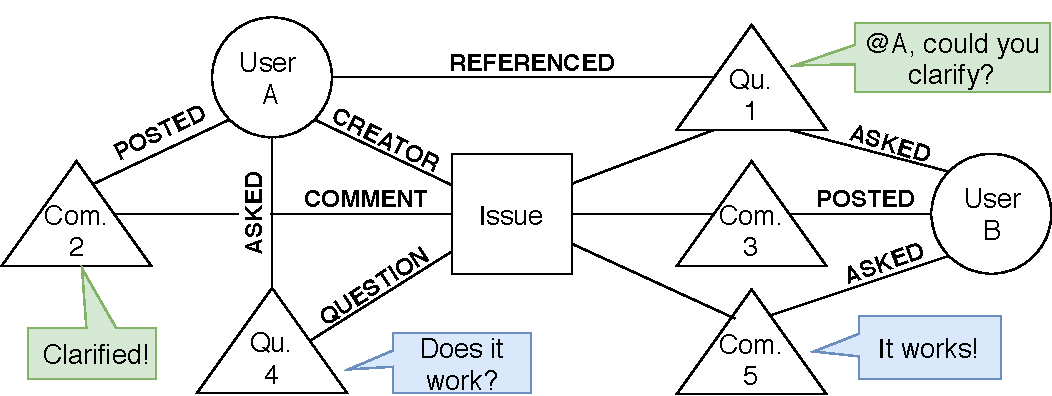
\includegraphics[width=\linewidth]{img/rstg.pdf}
	\caption{Requirements Socio-Technical Graph}
	\label{fig:rstg}
\end{figure}

The next step to creating patches in this network is to build a requirements socio-technical graph (RSTG) so that we can inspect the topology of the network using graph theory concepts. By manually inspecting common interactions, we are able to define the nodes and edges in our network topology. Consider the following example: Figure \ref{fig:rstg} is a subgraph from the IMMUNANT project, showing two questions and their answers. User A created the issue. User B, the forager, commented on the issue (Qu. 1), asking User A for clarification by referencing them in the comment. User A commented on the issue (Com. 2), providing the clarification. In another foraging interaction, User A, now the forager, commented on the issue (Qu. 4), and User B responded (Com. 5). 

Contemporary approaches to requirements traceability are either artifact-based (e.g., trace retrieval) and would consider only the comments and issues~\cite{ICSE15}, or are driven by social roles ~\cite{ICSE29}. However, this interaction and many like it indicated to us that we should represent our environment with comments, issues, and social roles as visible in Figure \ref{fig:rstg}. While some relationships could be considered as unidirectional, e.g., a user posting a comment, the comment also serves as a bridge connecting the issue to the user, who is knowledgeable on the issue. We therefore elected to encode the network as an undirected graph.

\subsection{Properties of Requirements Socio-Technical Graphs in Information Foraging}

We now tie our RSTGs to information foraging theory. When a forager asks a question, like the ones in Figure \ref{fig:rstg}, what path might they typically follow to the user who will provide the answer, gathering information on their prey along the way? By analyzing the paths connecting question nodes and answer nodes in the RSTG generated for each question, we identified recurring patterns connecting traceability questions with answers. The patterns are organized by degrees of socio-technical separation, which we define as the minimum number of edges to be traversed between two nodes. 

\subsubsection{One or Two Degrees of Separation}
More than three-quarters of answers to our 111 questions are within two degrees of the question. Thirty-one percent of answers were provided by users one degree away: either the asker referenced the user who will answer the question, or the asker themselves answered the question. Recall that when a user is referenced in a comment, they are connected to the comment. Fifty-five percent of answers were provided by users two degrees away: these users were the Creators or Assignees of the issue.

\subsubsection{Collaborators and Contributors\textemdash Three or Four Degrees} 
Eleven percent of our answers came within 3 degrees of separation; most of these answers fell within two classes that we called \textit{Frequent Collaborators} or \textit{Frequent Contributors}. Frequent Collaborators were users who were not connected to the issue, but were connected to the person asking. Frequent Contributors were users who commented or asked questions one or more times on an issue. Users A and B in Figures \ref{fig:rstg} and \ref{fig:rstg-sa} are Frequent Contributos, connected by their multiple comments on the issue. The remaining 3\% of answers, four degrees away, were Frequent Collaborators of the Creator or Assignee.

\subsubsection{Unconnected Users}
The final pattern observed was one instance of an answer unconnected from the graph of the project. At the time the question was asked, the user who will eventually answer the forager's traceability question was not yet connected to the project by the relationships we chose to express as edges. 

It appears, from these classes, that a substantial amount of traceability foraging takes place in four-or-less degrees of separation. Seeking to apply information foraging to traceability, one could simply present all nodes within four degrees of the question as a patch where the forager might seek to understand their question. This would satisfy our requirement of encoding frequently-traversed foraging paths into a patch. However, these patches are extremely large. Including all nodes within 2 degrees of separation produced patches with a mean size of 427 nodes. Including all within 4 degrees produced patches with a mean size of 2186 nodes. With some notion of relatedness, however, these patches could be made smaller without losing relevant information.

% =============================================================
% == Patches ==================================================
% =============================================================
\section{Creating Socio-Technical Patches for Information Foraging}
In order to create smaller patches which still contain the described relationships, we turn to the foraging concept of scent, which we define, following WUFIS and PFIS, as the ``inferred relatedness of a cue to the prey, as measured by amount of activation from a spreading activation algorithm''. We define ``relatedness'' in our domain as the amount of knowledge that a user has on an information artifact; this amount is encoded as weight on the edge connecting a user to the artifact. Note that, to support our implementation of spreading activation, a lower weight represents a more powerful connection.

Our strongest connections are Comments/Questions to Issues (weight = 1); they are directly part of the traceability history of an issue. Next, the Creator and Assignee have a high degree of knowledge on a given issue, answering 55\% of questions, though an issue can develop without the supervision of the creator or assignee (weight = 2). Next, the user who wrote the comment has determined that the referenced user should have strong knowledge on the comment (weight = 2). Finally, Comments' and Questions' connections to users are given the lowest weight (weight = 3, 4) because the user commenting or asking is not guaranteed to have knowledge on the issue to the same degree as Creator or Assignee. Figure \ref{fig:rstg-sa} shows an RSTG with these weights applied.

With weight defining the relatedness between two given nodes, a given node's relatedness to the forager's information need can be determined with spreading activation. Our variant of spreading activation starts at the question-node. The question's activation is set to 1. Then, surrounding nodes are traversed, and activation is spread from their predecessors. Spreading activation traditionally has each node firing to its successors; our predecessor variant exhibits greater decay while still producing useful networks.

\begin{figure}[ht]
	\centering
	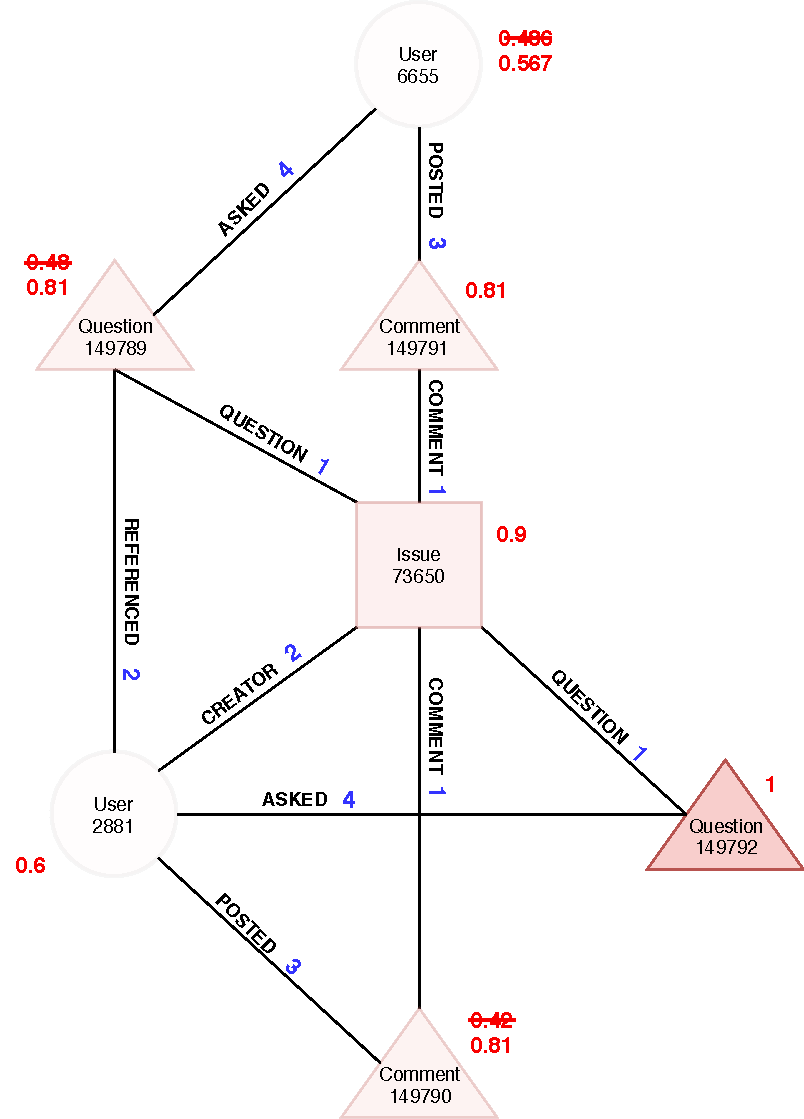
\includegraphics[width=\linewidth]{img/RSTG-SA.pdf}
	\caption{Spreading Activation Applied to an RSTG (Without Frequency Bonus)}
	\label{fig:rstg-sa}
\end{figure}

If a node has no activation yet, the activation is simply spread to the new node, decaying more if the weight value is higher. However, if a node already has activation, the higher activation value is spread. This can be seen in Figure \ref{fig:rstg-sa}. Finally, in order to incentivize frequency (in order to promote the Frequent Collaborator and Frequent Contributor patterns), if a node already has activation (i.e., the node has an existing relationship to the question), a percentage of that existing activation is added to the new activation.

By grouping together nodes with high activation, a patch with nodes related by the relationships described previously will be created. To do this, though, a threshold of ``high'' activation must be defined. Earlier, creating patches by simply enclosing all nodes within four degrees of separation was proposed, because all answers in our dataset fell within four degrees. We now consider those answers' activations. Examining graphs of the classes discussed earlier, with spreading activation completed, reveals that a forager setting the cutoff at 0.45 would include 100\% of results, just like 4 degrees. We could set the cutoff as high as 0.72 and still include 84\% of results.

\section{Results and Analysis}
Considering just these two extreme cutoffs, we find smaller patches than 4 degrees' mean of 2186 nodes: including all nodes with activation $\geq$ 0.45, we have patches of mean size 1281.2, and $\geq$ 0.72 yields patches of just mean size 7.4. Statistically comparing 4 Degrees and Activation $\geq$ 0.45, we conclude that the two sets are non-identical (t = 10.901, p-value $<$ 0.01). A similar test for Activation $\geq$ 0.45 and $\geq$ 0.72 reaches the same conclusion (t = 9.6481 p-value $\geq$ 0.01). In other words, each cutoff has significantly smaller patches than the previous. 

While patch sizes at cutoff activation $\geq$ 0.45 are still too big for timely foraging, patch sizes at $\geq$ 0.72 are reasonable. That being said, $\geq$ 0.72 patches frequently do not include the answer node for three or four degree of separation relationships. However, within these patches, we believe that foragers would still find information relevant to their information need.

Figure \ref{fig:rstg-sa} serves as a practical example of both the mechanism of the algorithm and a tradeoff to consider. Figure \ref{fig:rstg-sa} is a network with a cutoff set to $\geq$ 0.56\textemdash a cutoff chosen for its inclusion of many Frequent Contributors. Indeed, it was a Frequent Contributor that answered User A's question; User B had commented twice on the issue already. While the question (``Does it work?'') was a pointed request, asking for a specific piece of information, the patch generated by the request yields not only the user who will answer the request, but also related traceability information. 

Figure \ref{fig:rstg-sa} also demonstrates a limitation of the algorithm in its current state. Other implementations of spreading activation begin from one or more nodes; we could have started the activation from the question \textit{and} the asking user. We chose to include only the question node, as to avoid superfluous information from the asking user's connections. In this case, though, had we included User A as an initial node for activation, the algorithm would have assigned higher activations to the direct collaboration between User B and User A (User A--Question 1--User B). This collaboration was key to the traceability history of the issue.


% =============================================================
% == Implications =============================================
% =============================================================
\section{Implications}
Piorkowski and his colleagues~\cite{navValueCost} codified the fundamental challenges faced by software developers when foraging in the information environment. We believe that our socio-technical approach can help directly address the challenge of ``prey in pieces'' where the foraging paths were too long and disconnected by different topologies. By explicitly integrating humans in the underlying topology, information foragers can exploit a richer set of relationships.

Codebook~\cite{codebook10} confirmed that the small-world phenomenon~\cite{Chakrabarti-CSUR06} was readily observed in the socio-technical networks built from the software repositories. Our findings suggested that RSTGs are even smaller with relevant nodes surrounded in four-or-less degrees of separation from the traceability forager's question. Meanwhile, our results revealed several common relationships and their compositions. In light of the recent work on collecting practitioners' natural-language requirements queries (e.g.,~\cite{Pruski-REJ15, Lohar-REFSQ16, Malviya-RE17}), the patterns uncovered by our study could be used to better classify and answer project stakeholders' traceability needs.

Automated requirements traceability tools have been built predominantly by leveraging text retrieval methods~\cite{ICSE15}. These tools neglect an important factor\textemdash familiarity\textemdash which we find plays a crucial role in tracking the life of a requirement. Our results here are to be contrasted with the empirical work carried out by Dekhtyar \emph{et al.}~\cite{Dekhtyar-RE11} showing that experience had little impact on human analysts' tracing performance. While a developer's overall background may be broad, we feel that the specific knowledge about the subject software system and the latent relationships established with project stakeholders do play a role in requirements tracing. Automated ways of inferring a developer's knowledge degree (e.g.,~\cite{Fritz-TOSEM14}) would be valuable when incorporated in traceability tools.


% =============================================================
% == Conclusion ===============================================
% =============================================================
\section{Conclusion and Future Work}
By considering common relationships connecting a requirements traceability question to its answer, and encoding these relationships into a spreading activation algorithm, we were able to delineate patches for use in understanding context surrounding requirements traceability questions in a socio-technical environment. In this process, we found that traceability questions were answered by users within four degrees of socio-technical separation; these users were typically Frequent Collaborators of the forager or of the creator/assignee of the issue, or Frequent Contributors to the issue. Encoding these relationships as parameters to a spreading activation algorithm resulted in patches of nodes that a forager could traverse, searching for their answer. While simply creating patches including all nodes within four degrees of socio-technical separation would include all answers, the addition of spreading activation created significantly smaller patches.

This method can further be extended within the requirements traceability realm. With only three node types, we were able to generate these patches. With a higher diversity of information, such as code artifacts and commits, or semantic similarity, more nuanced relationships could be determined. Future work could be conducted on the implementation of the algorithm itself, too. Our parameters were set through observation and trial and error. More sophisticated statistical analyses could help better set these parameters. Our method only suggested the first patch for foraging; in reality, a forager will go through several patches in search of their prey. To accommodate this pattern, this work could be extended to multiple-patch creation. 

Finally, we determined nodes and edges by thoughtfully examining our environment. While the exact node and edge types would be different, applying the foundation of our design thinking and methods to new domains would create socio-technical graphs where spreading activation can provide relevant and small patches like ours. 

\section*{Acknowledgment}
The work is funded by the U.S. NSF Grant CCF-1350487.

\newpage
\balance
\bibliographystyle{IEEEtran}
\bibliography{VLHCC18-bib} 

\end{document}